\section{Effectiveness}

\begin{figure}[p]
  \centering
  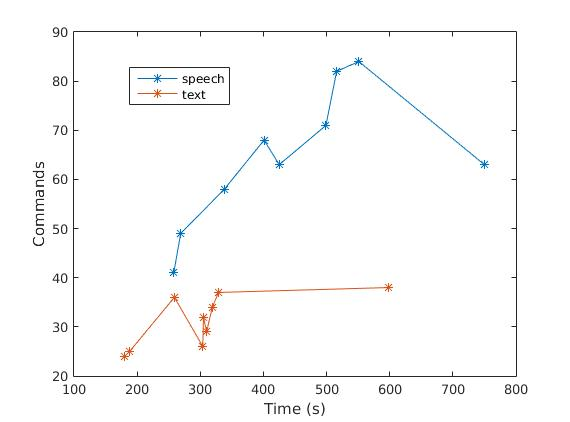
\includegraphics[width=0.8\textwidth]{images/time_cmd.jpg} %width=0.8\textwidth scales the image down to 80 percent of the text-width. Keeps the ratio.
  \caption{Bladiblala}\label{time_cmd}
\end{figure}

\subsection{Timescale}

\begin{table}[h!]
  \centering
  \begin{tabular}{ccc}
    \toprule
    Speech &   & Text\\
    \midrule
    445.22 &   & 310.22\\
    \bottomrule
  \end{tabular}
  \caption{Average Time}\label{avg_time}
\end{table}

\subsection{Commands}
Compare with ideal.

This is how you refer to table \ref{avg_cmd} or a graph. You look at the label. See comment in code.

\begin{table}[h!]
  \centering
  \begin{tabular}{ccc}
    \toprule
    Speech &   & Text\\
    \midrule
    64.33 &   & 31.22\\
    \bottomrule
  \end{tabular}
  \caption{Average Commands}\label{avg_cmd} % OMG LOOK HERE!!!
\end{table}

\section{Ease of Use}
%OBS!!!! MAYBE DESCRIPTION OF IDEAL SHOULD BE DESCRIBED SOMEWHERE ELSE
When the user played the game, the amount of commands used was recorded. A command is the entire sentence the user inputted into the game. To have something to compare to, the game was played by us to record what would be the minimum amount of commands needed to be used given that the player would have a lot of luck, or the ``ideal'' play-session. The rules used was that when entering a room, ``check room'' were inputted to get the description. No item in the room were checked, just taken or used, unless the puzzle involve looking at an item (such as a note). The result can be seen in figure \ref{ideal_cmd} where amount of commands users used is compared to the ideal for each game. In the text-version there is roughly 2 times the amount of commands as in the ideal, while in the speach-version it is about 4 times.

\begin{figure}[p]
  \centering
  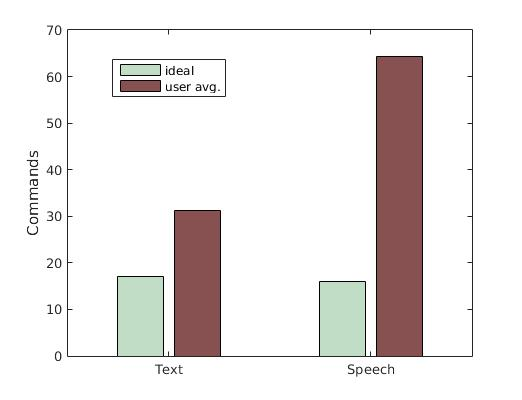
\includegraphics[width=0.8\textwidth]{images/ideal_cmd.jpg}
  \caption{Bladiblala}\label{ideal_cmd}
\end{figure}

\subsection{English Confidence}
Each user had to rate their spoken and written english between 1-5, where 1 is not good and 5 is fluent. These users were divided into groups and the average amount of commands, time and score were calculated for each group. The result for the amount of commands can be seen in figure \ref{eng_cmd}. 
\begin{figure}[p]
  \centering
  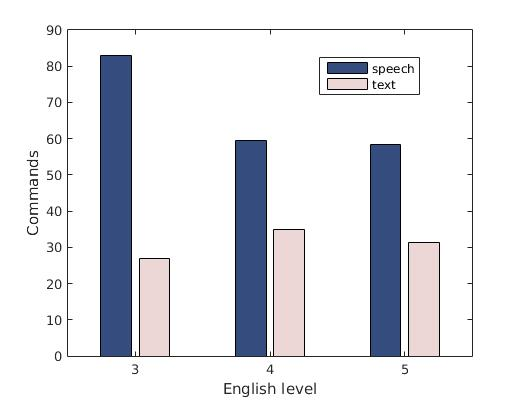
\includegraphics[width=0.8\textwidth]{images/english_cmd.jpg}
  \caption{Bladiblala}\label{eng_cmd}
\end{figure}
The time is put in seconds and is shown in figure \ref{eng_time}.
\begin{figure}[p]
  \centering
  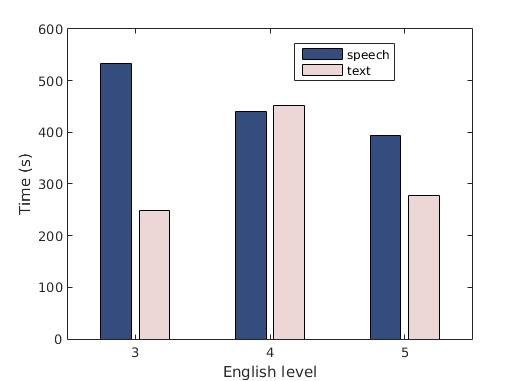
\includegraphics[width=0.8\textwidth]{images/english_time.jpg}
  \caption{Bladiblala}\label{eng_time}
\end{figure}
The score from the System Usability Scale in relation to the english level is displayed in figure \ref{eng_score}.
\begin{figure}[p]
  \centering
  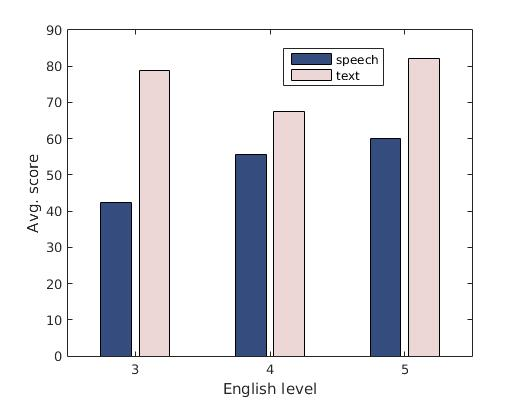
\includegraphics[width=0.8\textwidth]{images/english_score.jpg}
  \caption{Bladiblala}\label{eng_score}
\end{figure}

%\subsection{User Former Experience}

\section{Satisfaction (SUS)}
Figure \ref{sus_table} shows the average answer on each question after they have been converted according to formulae \ref{eq:convert} in section \ref{sec:sus}. 
\begin{figure}[p]
  \centering
  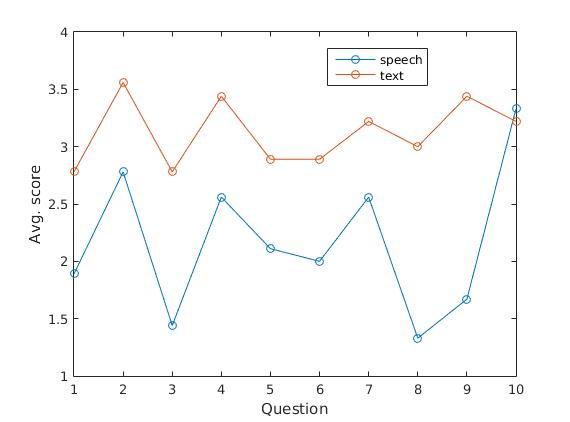
\includegraphics[width=0.8\textwidth]{images/sus.jpg}
  \caption{Bladiblala}\label{sus_table}
\end{figure}

The total average score as calculated in formulae \ref{eq:sum} for each version can be seen in table \ref{tot_score}.
\begin{table}[h!]
  \centering
  \begin{tabular}{ccc}
    \toprule
    Speech &   & Text\\
    \midrule
    54.17 &   & 78.06\\
    \bottomrule
  \end{tabular}
  \caption{Caption for the table.}\label{tot_score}
\end{table}

satisfaction